\documentclass[aspectratio=169]{beamer}
\usepackage[backend=bibtex,style=authoryear]{biblatex}
\bibliography{mscript_mck_full}
% \setbeamertemplate{bibliography item}{}
\AtBeginBibliography{\tiny}
\usepackage{lmodern,graphicx,amsthm,amsmath,amssymb,braket,textpos}
\usetheme{focus}
\newcommand{\focus}[1]{\textcolor{blue}{\textbf{#1}}}
\newcommand{\cen}[1]{\begin{center}{#1}\end{center}}
\setbeamercolor{itemize/enumerate body}{fg=gray}
\definecolor{maroon}{HTML}{540000}

\renewcommand{\thefootnote}{}
\renewcommand*\footnoterule{}
\setbeamercolor{footnote}{fg=blue}
\setbeamerfont{footnote}{size=\small}

\AtBeginSection[]{
\begin{frame}[noframenumbering]
  \vfill
  \centering
  \begin{beamercolorbox}[sep=8pt,center,rounded=true]{title}
    \usebeamerfont{title}\insertsectionhead\par%
  \end{beamercolorbox}
  \vfill
\end{frame}
}

\title{
\LARGE{Unveiling the Kondo cloud: \\
unitary RG study of the\\
Kondo model}
}
\subtitle{}
\date{\today}
\author{\large Anirban Mukherjee \inst{1}, Abhirup MUkherjee \inst{1}, N. S. Vidhyadhiraja \inst{2},\\ A. Taraphder \inst{3} \and Siddhartha Lal \inst{1}}


\institute{\small\inst{1} Department of Physical Sciences,IISER Kolkata\\ 
\inst{2} Theoretical Sciences Unit, JNCASR \\
\inst{3} Department of Physics, IIT Kharagpur}

\date{\large\today}

\begin{document}

\begin{frame}[noframenumbering]
\maketitle
\begin{textblock*}{2cm}(9.4cm,-8.7cm)
	\includegraphics[width=150pt]{figures/title_fig.png}
\end{textblock*}
\end{frame}

\section{The Model}
\begin{frame}[noframenumbering]{The Model}
\only<+>{\centering
\scalebox{1.5}{
	\(\mathcal{H} = \sum_{k\sigma}\epsilon_k \hat n_{k\sigma} + J \vec{S}_d\cdot\vec{s}, ~ ~ ~ ~ ~ \vec s \equiv \sum_{kk^\prime,\alpha,\beta}\vec \sigma_{\alpha\beta}c^\dagger_{k\alpha}c_{k^\prime\beta}
\)
}
\vspace*{\fill}

\begin{figure}
\hspace*{\fill}
\includegraphics[width=0.35\textwidth]{figures/2dKondoTN.pdf}
\hspace*{\fill}
\includegraphics[width=0.4\textwidth]{figures/kondoSetup.pdf}
\hspace*{\fill}
\end{figure}
}
\only<2-5>{
\begin{minipage}{0.6\textwidth}
\begin{itemize}[<+-|alert@+>]
\item Kondo coupling \(J\) renormalises to infinity\\[10pt]
\item low energy phase of metal is local Fermi liquid\\[10pt]
\item \(\chi\) constant at low temperatures, \(C_v\) linear\\[10pt]
\item thermal quantities functions of single scale \(T/T_K\)\\[10pt]
\end{itemize}
\end{minipage}
\begin{minipage}{0.35\textwidth}
	\only<2-3>{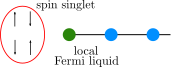
\includegraphics[width=\textwidth]{figures/cloud_lFL.pdf}}
	\only<4-5>{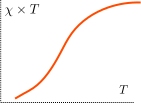
\includegraphics[width=\textwidth]{figures/chi_schematic.pdf}}
\end{minipage}
\footcite{anderson1969exact,anderson1970,wilson1975,andreiKondoreview,andrei_kondo,wiegmann_kondoexact_1981}
}
\end{frame}

\section{What's left to understand?}
\begin{frame}[noframenumbering]{What's Left To Understand?}
  
\begin{itemize}[<+-|alert@+>]
	\item Finite \(J\) effective Hamiltonian at fixed point
	\vspace*{20pt}
	\item Hamiltonian for the itinerant electrons forming the \textbf{macroscopic singlet}
	\vspace*{20pt}
	\item Nature of correlations inside the Kondo cloud: \textbf{Fermi liquid vs off-diagonal}
	\vspace*{20pt}
	\item Behaviour of \textbf{many-particle entanglement} and many-particle correlation under RG flow
\end{itemize}

\end{frame}

\section{The Unitary Renormalization Group Method}
\begin{frame}[noframenumbering]{The Unitary Renormalization Group Method}
\footcite{anirbanurg1,anirbanurg2}

\centering
\textbf{\large The General Idea}
\only<1-3>{
\begin{minipage}{0.8\textwidth}
\begin{itemize}[<+-|alert@+>]
	\item Apply unitary many-body transformations to the Hamiltonian\\[10pt]
	\item Successively decouple high energy states\\[10pt]
	\item Obtain sequence of Hamiltonians and hence scaling equations
\end{itemize}
\end{minipage}
}
\begin{minipage}{0.15\textwidth}
\begin{figure}
	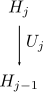
\includegraphics[width=0.7\textwidth]{figures/urg_schematic.pdf}
\end{figure}
\end{minipage}
\end{frame}
\begin{frame}[noframenumbering]{The Unitary Renormalization Group Method}
\footcite{anirbanurg1,anirbanurg2}
\centering
\only<+>{
\large{\textbf{Select a UV-IR Scheme}}
\vspace*{\fill}

\begin{minipage}{0.5\textwidth}
\centering
\textbf{\color{red} UV shell}
\begin{gather*}
	\vec k_N ~~ \left(\text{zeroth RG step}\right)\\
\vdots\\ 
\vec k_j ~ ~ \left(j^\text{th} \text{ RG step}\right) \\
\vdots\\
\vec k_1 ~ ~ \left(\text{Fermi surface}\right)
\end{gather*}
\textbf{\color{maroon} IR shell}
\end{minipage}
\hspace*{\fill}
\begin{minipage}{0.4\textwidth}
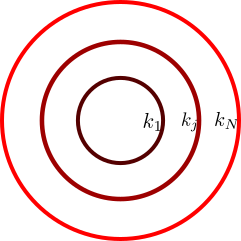
\includegraphics[width=0.9\textwidth]{figures/uv_ir_scheme.pdf}
\end{minipage}
\vspace*{\fill}
}

\only<+>{
\vspace*{-20pt}
\large{\textbf{Write Hamiltonian in the basis of \(\vec k_j\)}}
\vspace*{\fill}

\begin{minipage}{0.4\textwidth}
	\[H_{(j)} = H_1 \hat n_j + H_0 \left(1 - \hat n_j\right) + c^\dagger_j T + T^\dagger c_j\]
\[
 {2^{j-1} \text{-dim.}} \longrightarrow \begin{cases}
	H_1, H_0 \longrightarrow \text{diagonal parts}\\
V \longrightarrow \text{off-diagonal part}
\end{cases}
\]
\end{minipage}
\hspace*{\fill}
\begin{minipage}{0.5\textwidth}
\begin{figure}
	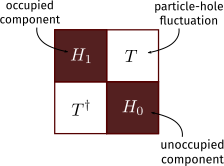
\includegraphics[width=0.9\textwidth]{figures/urg_ham.pdf}
\end{figure}
\end{minipage}
}
\only<+>{
\vspace*{-10pt}
\large{\textbf{Rotate Hamiltonian and kill off-diagonal blocks}}

\vspace*{\fill}

\begin{minipage}{0.45\textwidth}
	\[H_{(j-1)} = U_{(j)} H_{(j)} U_{(j)}^\dagger\]
	\[U_{(j)} = \frac{1}{\sqrt 2}\left(1 - \eta_{(j)} + \eta_{(j)}^\dagger\right) \]
	\[ \eta^\dagger_{(j)} = \frac{1}{\hat \omega_{(j)} - H_D}c^\dagger_j T \Bigg \} \rightarrow {\text{many-particle}\atop{\text{rotation}}}\]
\end{minipage}
\hspace*{\fill}
\begin{minipage}{0.5\textwidth}
\begin{figure}
	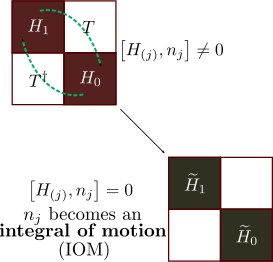
\includegraphics[width=0.8\textwidth]{figures/urg_rot.pdf}
\end{figure}
\end{minipage}
}

\only<+>{
\vspace*{-20pt}
\large{\textbf{Repeat with renormalised Hamiltonian}}
\vspace*{\fill}

\begin{minipage}{0.53\textwidth}
	\[H_{(j-1)} = \widetilde H_1 \hat n_j + \widetilde H_0 \left(1 - \hat n_j\right)\]
	\[\widetilde H_1 = H_1 \hat n_{j-1} + H_0 \left(1 - \hat n_{j-1}\right) + c^\dagger_{j-1} T + T^\dagger c_{j-1}\]
\end{minipage}
\hspace*{\fill}
\begin{minipage}{0.45\textwidth}
\begin{figure}
	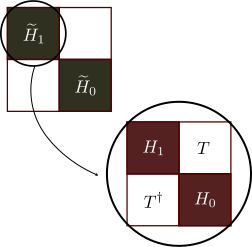
\includegraphics[width=\textwidth]{figures/urg_next.pdf}
\end{figure}
\end{minipage}
}

\only<+>{
\vspace*{-20pt}
\large{\textbf{RG Equations and Denominator Fixed Point}}

\vspace*{\fill}

\[ \Delta H_{(j)} = \left(\hat n_j - \frac{1}{2}\right) \left\{c^\dagger_j T, \eta_{(j)}\right\} \]

\[\eta^\dagger_{(j)} = \frac{1}{\hat \omega_{(j)} - H_D}c^\dagger_j T\] 

\[\text{\bf \color{maroon}Fixed point:}~ ~ ~\hat \omega_{(j^*)} - \left(H_D\right)^* = 0\]
}
\end{frame}

\begin{frame}[noframenumbering]{The Unitary Renormalization Group Method}
\centering
\vspace*{-20pt}
\large{\textbf{Novel Features of the Method}}

\vspace*{\fill}

\hspace*{-20pt}
\begin{minipage}{0.65\textwidth}
\begin{itemize}[<+-|alert@+>]
	\item Quantum fluctuation energy scale \(\omega\)
	\item Finite-valued fixed points for finite systems
	\item Spectrum-preserving unitary transformations
	\item Tractable low-energy effective Hamiltonians
\end{itemize}
\end{minipage}
\hspace*{\fill}
\begin{minipage}{0.3\textwidth}
	\[H_{(j-1)} = U_{(j)} H_{(j)} U_{(j)}^\dagger\]
	\[U_{(j)} = \frac{1}{\sqrt 2}\left(1 - \eta_{(j)} + \eta_{(j)}^\dagger\right) \]
	\[ \eta^\dagger_{(j)} = \frac{1}{\hat \omega_{(j)} - H_D}c^\dagger_j T\]
	\[ \Delta H_{(j)} = \left(\hat n_j - \frac{1}{2}\right) \left\{c^\dagger_j T, \eta_{(j)}\right\} \]
\end{minipage}
\end{frame}


\section{URG of the Kondo Model}
\begin{frame}[noframenumbering]{URG of the Kondo Model}
	\centering
	\textbf{\large RG Equation, Fixed Point Hamiltonian \& Phase Diagram}

\vspace*{\fill}

\hspace*{-10pt}
	\only<1>{
	Assumption:  isotropic energy surfaces: \(\epsilon_{\vec k_j} \equiv D_j\)

}
\begin{minipage}{0.35\textwidth}
		\centering
\only<1-4>{
	\[\Delta J_{(j)} = \frac{n_j ~ J_{(j)}^2 ~ \left(\omega_{(j)} - \frac{D_j}{2}\right)}{\left(\omega_{(j)} - \frac{D_j}{2}\right)^2 - \frac{1}{16}J_{(j)}^2}\]
	\[ J^* = 4\left(\omega^* - \frac{1}{2}D^*\right)\]
	\[D^* \longrightarrow \text{ emergent window}\]
}
\end{minipage}
	\only<1>{
		\\[10pt]
		\color{maroon} For \(J_{(j)} \ll D_j\), we recover weak-coupling form: \(\frac{\Delta J_{(j)}}{\Delta \ln D_j} \sim n_j ~ J_{(j)}^2\)
		\footcite{anderson1970}
	}
\only<2-4>{
\hspace*{\fill}
\begin{minipage}{0.6\textwidth}
	\centering
	\[\omega_{(j)} > \frac{D_j}{2}\]
	\only<2>{
		\vspace*{-10pt}
	\[K_{(j)} = J_{(j)}\left(\omega^* - \frac{1}{2}D^*\right)^{-1}\]
	\includegraphics[width=0.8 \textwidth]{figures/RG_flow.pdf}
}
	\only<3>{
	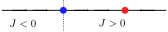
\includegraphics[width=\textwidth]{figures/kondo_phase.pdf}
	\begin{itemize}
		\item Decay towards FM fixed point for \(J<0\)
		\item Attractive flow towards AFM fixed point for \(J>0\)
	\end{itemize}
}
	\only<4>{
		\[H^* = \underbrace{\sum_{k,\sigma}\epsilon_{k}\hat{n}_{k\sigma} ~ + ~ J^* \vec{S}\cdot \vec{s}_<}_\text{emergent window} ~ + ~\underbrace{\sum_{j=j^*}^N J^{j}S^{z}s^{z}_{j}}_\text{integrals of motion}\]
}
\end{minipage}
}
\end{frame}

\end{document}

\section{RG Equations, Their Features and Fixed Points}
\begin{frame}[noframenumbering]{RG Equations}
\[
\Delta U = 4|V|^2 \left[\frac{1}{\omega - \frac{1}{2}D + \frac{U}{2} + \frac{1}{2}J}  - \frac{1}{\omega - \frac{1}{2}D - \frac{U}{2} + \frac{1}{2}K}\right] + \sum_{k<\Lambda_j} \frac{3}{4}\frac{K^2 - J^2}{\omega - \frac{1}{2}D + \frac{1}{4}J + \frac{1}{4}K}
\]

\[
	\hspace*{-10pt}\Delta V = \frac{V K}{16}\left(\frac{1}{\omega - \frac{1}{2}D - \frac{U}{2} + \frac{1}{2}K} + \frac{1}{\omega - \frac{1}{2}D + \frac{1}{4}J + \frac{1}{4}K} \right) - \frac{3VJ}{4}\left( \frac{1}{\omega - \frac{1}{2}D + \frac{U}{2} + \frac{1}{2}J} + \frac{1}{\omega - \frac{1}{2}D + \frac{1}{4}J + \frac{1}{4}K} \right)
\]

\[
\Delta J = - J^2\left(\omega - \frac{1}{2}D + \frac{1}{4}J + \frac{1}{4}K\right)^{-1}
\]

\[
\Delta K = - K^2\left(\omega - \frac{1}{2}D + \frac{1}{4}J + \frac{1}{4}K\right)^{-1}
\]
\end{frame}

\begin{frame}[noframenumbering]{Passage to Poor Man's Scaling Results}
\only<+>{
	\cen{\textbf{Symmetric SIAM}}
\hspace*{0.15\textwidth}
\begin{minipage}{0.25\textwidth}
\begin{itemize}
	\item \(J=0, K=0\)
	\item \(\omega = -\frac{D}{2}\)
	\item \(U = -\frac{\epsilon_d}{2} \ll D\)
\end{itemize}
\end{minipage}
\begin{minipage}{0.2\textwidth}
	{\LARGE \[\longrightarrow\]}
\end{minipage}
\begin{minipage}{0.25\textwidth}
	\centering
	\Large \(\delta U = \delta V = 0\)
\end{minipage}
\hspace*{0.14\textwidth}
}

\only<+>{
	\cen{\textbf{Asymmetric SIAM}}
\hspace*{0.15\textwidth}
\begin{minipage}{0.25\textwidth}
\begin{itemize}
	\item \(J=0, K=0\)
	\item \(\omega = -\frac{D}{2}\)
	\item \(U \gg D \gg \epsilon_d\)
\end{itemize}
\end{minipage}
\begin{minipage}{0.2\textwidth}
	{\LARGE \[\longrightarrow\]}
\end{minipage}
\begin{minipage}{0.25\textwidth}
	\centering
	\Large\(\delta U = \delta V = 0\)\\[10pt]
	\(\delta \epsilon_d = \frac{\Delta}{\pi}\delta \ln{D}\)
\end{minipage}
\hspace*{0.14\textwidth}
}
\footcite{haldane,Jefferson}
\end{frame}

\begin{frame}[noframenumbering]{Fixed Points}
\begin{minipage}{0.6\textwidth}
\only<+>{
	\begin{itemize}
		\item \(J=K=0 \longrightarrow \Delta V = 0\)
			\vspace*{20pt}
		\item \(J,K,V=0^+ \longrightarrow \left(V^*, J^*, K^*\right)=\text{large}, U^*=0\)
			\begin{itemize}
				\item \focus{strong-coupling fixed point}
			\end{itemize}
	\end{itemize}
}
\only<+>{
	\begin{itemize}
		\item \(J=K=V=0 \longrightarrow \text{all couplings marginal}\)
			\begin{itemize}
				\item line of fixed points on y-axis
			\end{itemize}
			\vspace*{20pt}
		\item \(U=0^+ \longrightarrow \text{\focus{local moment fixed point}}\)
			\begin{itemize}
				\item ground-state is a decoupled impurity spin
			\end{itemize}
	\end{itemize}
}
\end{minipage}
\begin{minipage}{0.38\textwidth}
	\centering
	\includegraphics[width=\textwidth]{figures/nrg_fpoints.png}
\end{minipage}
\end{frame}

\begin{frame}[noframenumbering]{Results: \(U>0, J>K\)}
\begin{minipage}{0.6\textwidth}
\cen{
	\includegraphics[width=\textwidth]{figures/UvsJ.pdf}
}
\end{minipage}
\begin{minipage}{0.39\textwidth}
\cen{
	\includegraphics[width=0.95\textwidth]{figures/U_vs_count.pdf}
	\includegraphics[width=0.95\textwidth]{figures/J_vs_count.pdf}
}
\end{minipage}
\end{frame}


\begin{frame}[noframenumbering]{Results: \(U<0, J<K\)}
	\vspace*{30pt}
\cen{
	\includegraphics[width=0.49\textwidth]{figures/U_vs_count_neg.pdf}
	\includegraphics[width=0.49\textwidth]{figures/K_vs_count_neg.pdf}
}
\end{frame}

\section{Low energy effective theory and ground state wavefunctions}
\begin{frame}[noframenumbering]{Results: Phase Diagram}
\cen{
	\def\svgwidth{0.75\columnwidth}
	\input{./phases_V_pres.pdf_tex}
}
\end{frame}

\begin{frame}[noframenumbering]{Results: Effective Zero-mode Hamiltonian}
	\vspace*{-30pt}
\cen{
	\Large\[H_{IR} = \epsilon_d^* \left( \hat n_{1 \uparrow} - \hat n_{1 \downarrow} \right) ^2 + V^*\sqrt{N^*}\sum_{\sigma}\left(c^\dagger_{1\sigma}c_{2\sigma} + \text{h.c.} \right) + J^*N^*\vec{S_1}\cdot\vec{S_2} + K^*N^*\vec{C_1}\cdot\vec{C_2}\]
}
\hspace*{-15pt}
	\begin{minipage}{0.5\textwidth}
	{\centering
	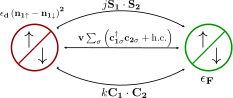
\includegraphics[width=\textwidth]{figures/two_site_problem.png}}
\end{minipage}
\hspace*{25pt}
\begin{minipage}{0.45\textwidth}{
	\centering
	\def\svgwidth{\columnwidth}
	\input{gstate_pres.pdf_tex}
	% \includegraphics[width=\textwidth]{figures/gstate_state.png}
}

\end{minipage}

\footcite{wilson,hrk-nrg,taraphder}

\end{frame}

% \begin{frame}[noframenumbering]{Results: Ground State}
% \begin{minipage}{0.65\textwidth}
% 	\[J > K, U>0\]
% \vspace*{-10pt}
% 	\[\ket{\Psi}_\text{GS} = c_-^s\left[\ket{\uparrow, \Downarrow} - \ket{\downarrow, \Uparrow}\right] + c_-^c\left[\ket{\uparrow, \Downarrow} + \ket{\downarrow, \Uparrow}\right]\]

% \vspace*{10pt}
% \begin{minipage}{0.65\textwidth}
% \begin{figure}[htpb]
% 	\centering
% 	\includegraphics[width=0.8\textwidth]{figures/cscc_q1.pdf}
% \end{figure}
% \end{minipage}
% \begin{minipage}{0.3\textwidth}
% 	\[ c_-^s \to 1\]
% 	\[ c_-^c \to 0\]
% \end{minipage}
% \[\ket{\Psi}_\text{GS} \sim \left[\ket{\uparrow, \Downarrow} - \ket{\downarrow, \Uparrow}\right]\]
% \end{minipage}
% \vline
% \begin{minipage}{0.34\textwidth}
% \[J < K, U<0\]
% \[\ket{\Psi}_\text{GS} = \left[\ket{\uparrow_c, \Downarrow_c} - \ket{\downarrow_c, \Uparrow_c}\right]\]
% \vspace*{0.6\textheight}
% \end{minipage}
% \end{frame}

\section{Impurity Susceptibilities and Impurity spectral function}
\begin{frame}[noframenumbering]{Results: Spin Susceptibility}
	\vspace*{-20pt}
	\[\chi_s = \lim_{B \to 0} \frac{\partial{m}}{\partial{B}}\]
\cen{
	\hspace*{-20pt}
	\includegraphics[width=0.48\textwidth]{figures/chi_T.pdf}
	\hspace*{25pt}
	\includegraphics[width=0.48\textwidth]{figures/chi.pdf}
}
\hspace*{20pt}\large{\(
\chi\left( T \to 0 \right) = \left(2j\right)^{-1} \hspace*{\fill} T_K \equiv \frac{2N^*}{\pi}\left(D^* - 2\omega\right)\hspace*{\fill} \left(\chi \times T\right) \left( T \to \infty \right) = \frac{1}{8}\)}

\footcite{wilson, hrk-nrg}
\end{frame}

\begin{frame}[noframenumbering]{Results: Charge Susceptibility}
	\vspace*{-15pt}
	\[\chi_c = \lim_{\mu \to 0} \frac{\partial{N}}{\partial{\mu}}\]
\cen{
	\hspace*{-20pt}
	\includegraphics[width=0.48\textwidth]{figures/chi_c.pdf}
	\hspace*{25pt}
	\includegraphics[width=0.48\textwidth]{figures/T_chi_c.pdf}
}
\large{\(
\chi_c \left(T \to 0\right)\big\vert_{K>J} = \frac{1}{2k} \hspace*{\fill} \left(\chi_c\times T\right)\left(T \to 0\right)\big\vert_{J>K} = 0 \hspace*{\fill} \left(\chi_c\times T\right)\left( T \to \infty \right) = \frac{1}{8}\)}

\footcite{taraphder,charge-kondo-Zitko}
\end{frame}

\begin{frame}[noframenumbering]{Results: Impurity Spectral Function}
	\(\mathcal{A(\omega)} = -\frac{1}{\pi}\text{Im }\left[G_{d d}^\sigma\left( \omega \right) \right]\) \hspace*{\fill} \(G_{d d}^\sigma\left(t\right) = -i\theta(t)\left<\left\{ c_{d\sigma}(t), c^\dagger_{d\sigma} \right\}\right>\)
\cen{
	\includegraphics[width=\textwidth]{figures/spec_func_merged_2.png}
}
\footcite{hewson,bulla_costi_nrg}
\end{frame}

\begin{frame}[noframenumbering]{Results: Spectral Function Renormalization}
	\(\mathcal{A(\omega)} = -\frac{1}{\pi}\text{Im }\left[G_{d d}^\sigma\left( \omega \right) \right]\) \hspace*{\fill} \(G_{d d}^\sigma\left(t\right) = -i\theta(t)\left<\left\{ c_{d\sigma}(t), c^\dagger_{d\sigma} \right\}\right>\)
\cen{
	\includegraphics[width=0.47\textwidth]{figures/spec_func_journey_one_marked.pdf}\hspace*{\fill}\includegraphics[width=0.45\textwidth]{figures/spec_func_journey_three_marked.pdf}
}
\end{frame}

\section{Entanglement measures and Topological Features of low energy theory}
\begin{frame}[noframenumbering]{Results: Kondo Cloud Hamiltonian}
	\vspace*{-10pt}
	\[H^*(\text{d, cloud}) \xrightarrow{\text{solve for bath Hamiltonian}} H^*_\text{cloud}\] 
	\[H^*_\text{cloud} = \overbrace{H^*_0}^\text{kinetic energy} + \overbrace{\sum_{kk^\prime\sigma\sigma^\prime}f_{kk^\prime}\hat n_{k\sigma}\hat n_{k^\prime\sigma^\prime}}^\text{Fermi liquid-type interaction} + \overbrace{\sum_{kk^\prime qq^\prime}F_{kk^\prime qq^\prime}c^\dagger_{k \uparrow}c^\dagger_{k^\prime \downarrow} c_{q \uparrow}c_{q^\prime \downarrow}}^\text{non-Fermi liquid-type interaction}\]
\begin{figure}[htpb]
	\centering
	\includegraphics[width=0.45\textwidth]{figures/Fkkqq.pdf}
\end{figure}
\end{frame}

\begin{frame}[noframenumbering]{Results: Reverse RG: Overview}
	\vspace*{\fill}
	\begin{figure}[htpb]
		\centering
		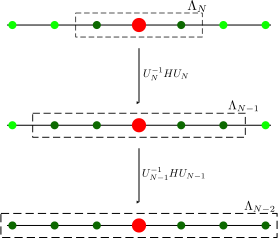
\includegraphics[width=0.5\textwidth]{figures/reverse-rg.png}
		\hspace*{\fill}
		\includegraphics[width=0.45\textwidth]{figures/rev-rg-bonds-diag.png}
	\end{figure}
	\vspace*{\fill}
\footcite{am_thesis}
\end{frame}

\begin{frame}[noframenumbering]{Results: Reverse RG: Mutual Information}
	\hspace*{\fill}	\(I(A:B) = S_A + S_B - S_{AB}\)\hspace*{\fill}\(S_A = -\text{Tr }\left[\rho_A \ln \rho_A\right]\)\hspace*{\fill}
	\begin{figure}[htpb]
		\centering
		\includegraphics[width=0.45\textwidth]{figures/mutI_ee.png}\hspace*{\fill}
		\includegraphics[width=0.45\textwidth]{figures/mutI_ed.png}
	\end{figure}
\end{frame}


\begin{frame}[noframenumbering]{Results: Reverse RG: Correlations}
	\begin{figure}[htpb]
		\centering
		\includegraphics[width=0.45\textwidth]{figures/corr_diag.png}\hspace*{\fill}
		\includegraphics[width=0.45\textwidth]{figures/corr_od.png}
	\end{figure}
\end{frame}

\begin{frame}[noframenumbering]{Results: Luttinger's Theorem}
	\hspace*{\fill}	{\Large \(\overbrace{N}^{\text{total no. of}\atop{\text{ particles}}} = \overbrace{P_{\text{Det }G_d}(\Gamma_<) + \frac{1}{2}P_{\text{Det }G_d}(\Gamma_0)}^{\text{no. of poles of}\atop{\text{imp. Greens func.}}} + \overbrace{V_L}^{\text{no. of poles of}\atop{\text{cbath Greens func}}}\)}\hspace*{\fill}
\begin{equation*}\begin{aligned}
	P_X(C) &\equiv \frac{1}{2\pi i}\oint_C dz \frac{\partial{\ln X}}{\partial{z}} &&=\text{no. of poles of } X \text{ enclosed by curve }C \\
	       &= \frac{1}{2\pi i}\oint_{X(C)} \frac{dX}{X} &&= \text{winding number of } X(C) \text{ around the origin}
\end{aligned}\end{equation*}
\begin{minipage}{0.4\textwidth}
	\begin{figure}[htpb]
		\centering
		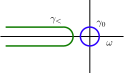
\includegraphics[width=0.9\textwidth]{figures/contours.png}
	\end{figure}
\end{minipage}
\hspace*{0.15\textwidth}
\begin{minipage}{0.4\textwidth}
	\begin{figure}[htpb]
		\centering
		\includegraphics[width=0.9\textwidth]{figures/wind_num.png}
	\end{figure}
\end{minipage}
\footcite{seki}
\end{frame}

\begin{frame}[noframenumbering]{Results: Luttinger's Theorem}
\begin{minipage}{0.6\textwidth}
\begin{figure}[htpb]
	\centering
	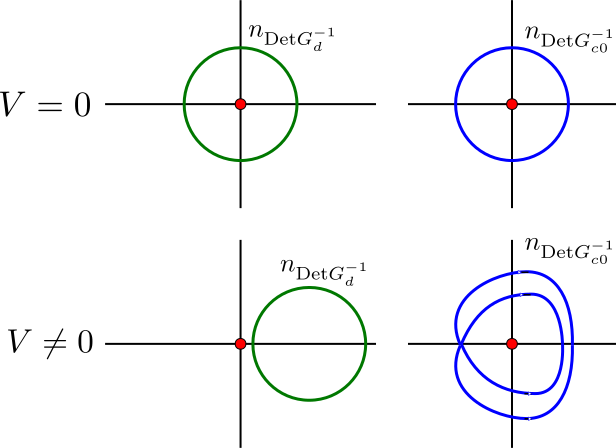
\includegraphics[width=0.75\textwidth]{figures/luttinger_top_change.png}
\end{figure}
\end{minipage}
\begin{minipage}{0.39\textwidth}
	\vspace*{5pt}
		{\large \[n_{\text{Det }G_d^{-1}} = 1\]
	\vspace*{45pt}
\[n_{\text{Det }G_d^{-1}} = 0\]}
\end{minipage}
\vspace*{10pt}
\cen{
	\Large
	\(V_L = V_L^0 + 1\)
}

\footcite{martin}
\end{frame}

\begin{frame}[noframenumbering]{Results: Local Fermi Liquid}
	\[H^* = \overbrace{J^* \vec{S_d}\cdot\vec{s} + K^* \vec{C_d}\cdot\vec{c} + V^* \left( c^\dagger_{d\sigma}c_{0\sigma} + \text{h.c.} \right)}^\text{solve exactly} + \overbrace{t\sum_{\left<i,j \right>}c^\dagger_{i\sigma}c_{j\sigma}}^\text{treat as perturbation}\]
	\hspace*{0.5\textwidth}$\Bigg\downarrow$ \(4^\text{th}\) fourth order pert.
	\[E_1^{(4)} = -\frac{16t^4}{3{J^*}^3}, E_2^{(4)} = -\frac{16t^4}{9{J^*}^3}\]
	\[H^* \sim J^* \vec{S_d}\cdot\vec{s} + K^* \vec{C_d}\cdot\vec{c} + V^* \left( c^\dagger_{d\sigma}c_{0\sigma} + \text{h.c.} \right) + \overbrace{\frac{t^4}{{J^*}^3} \hat n_{1 \uparrow}\hat n_{1 \downarrow}}^\text{local Fermi liquid}\]

\vspace*{-10pt}
\footcite{nozieres}
\end{frame}

\begin{frame}[noframenumbering]{Results: Wilson Ratio (\(T=0\))}
\vspace*{-10pt}
\cen{
	\text{thermal average:} \(\left<\hat n_{1 \uparrow}\hat n_{1 \downarrow}\right> \xrightarrow{\text{mean field}\atop \text{approximation}} \left<\hat n_{1 \uparrow}\right>\left<\hat n_{1 \downarrow}\right>\)\\[20pt]
\scalebox{1.5}{
	\(\epsilon_{k\sigma} = \epsilon_k^0 + \sum_q f_{kq}\left<n_{q\overline\sigma} \right>\)
}
}
\vspace*{\fill}
\hspace*{60pt}
\begin{minipage}{0.25\textwidth}
\begin{itemize}
	\item \(f_{\uparrow\uparrow} =0\)
	\item \(\chi_c(T\to 0) =0\)
\end{itemize}
\end{minipage}
\begin{minipage}{0.15\textwidth}
	\scalebox{2}{$\longrightarrow$}
\end{minipage}
\begin{minipage}{0.33\textwidth}
\begin{itemize}
	\item \(C_v(T\to 0) = \rho_\text{imp}T\)
	\item \(\chi_s(T \to 0) = 2\rho_\text{imp}\)
\end{itemize}
\end{minipage}
\hspace*{20pt}
\vspace*{\fill}
\cen{
	\scalebox{1.5}{
	$R = \frac{\chi_s}{\frac{C_v}{T}} = 2$
}
}

\footcite{hewsonp}
\end{frame}

\begin{frame}[noframenumbering]{Results: Relation between \(R\) and \(\Delta V_L\)}
	\only<1-3>{
	\hspace*{30pt}
	\begin{minipage}{0.4\textwidth}
		\begin{itemize}
			\item particle-hole symmetry
				\vspace*{5pt}
			\item strong-coupling fixed-point
				\vspace*{5pt}
			\item \(T=0\)
		\end{itemize}
	\end{minipage}
	\begin{minipage}{0.15\textwidth}
		\cen{
			\LARGE\(\longrightarrow\)
	}
	\end{minipage}
	\begin{minipage}{0.3\textwidth}
		\centering
		\(\frac{\chi_s}{C_v/T} = 1 + U\rho_\text{imp}(0)\)\\[10pt]
		\(\rho_\text{imp}(0) = \left(\pi\Delta\right)^{-1}\sin^2 \delta(0)\)\\[10pt]
		\(R = 1 + \sin^2 \delta(0)\)
	\end{minipage}
	\footcite{piers,hewson,phill}
}

\only<2-3>{
	\vspace*{30pt}
	\hspace*{30pt}
	\begin{minipage}{0.4\textwidth}
		\begin{itemize}
			\item Friedel's sum rule 
				\vspace*{5pt}
			\item scattering theory results
				\vspace*{5pt}
		\end{itemize}
	\end{minipage}
	\begin{minipage}{0.18\textwidth}
		\cen{
			\LARGE\(\longrightarrow\)
	}
	\end{minipage}
	\begin{minipage}{0.25\textwidth}
		\Large\(\frac{2}{\pi}\delta(0) = \tilde N = \Delta V_L\)
	\end{minipage}
}

\only<3>{
	\vspace*{15pt}
	\cen{
		\Large\(R = 1 + \sin^2 \left( \frac{\pi}{2} \Delta V_L \right) \)\\[10pt]
		\Large\(\Delta V_L = 1 \longrightarrow R = 2 \)
}
}
\end{frame}
% \only<1>{
% \begin{flalign*}
% 	\mathcal{H} = \overbrace{\sum_{k\sigma}\epsilon_k \hat n_{k\sigma} + \sum_{k\sigma}\left[V(k)c^\dagger_{k\sigma}c_{d\sigma} + \text{h.c.}\right] + \epsilon_d \sum_\sigma \hat n_{d\sigma} + U\hat n_{d\uparrow}\hat n_{d\downarrow}}^{SIAM}\\
%  + \underbrace{J \vec{S_d}\cdot \sum_{kq\alpha\beta}\vec{\sigma}_{\alpha,\beta}c^\dagger_{k\alpha}c_{q\beta}}_\text{spin-exchange}+ \underbrace{J \vec{C_d}\cdot \sum_{kq\alpha\beta}\vec{\sigma}_{\alpha,\beta}\psi^\dagger_{k\alpha}\psi_{q\beta}}_\text{isospin-exchange}
% \end{flalign*}
% }
% \only<2-3>{\Large{\textbf{RG Equations}}
% \only<2>{
% 	\vspace*{-15pt}
% 		\begin{equation*}\begin{aligned}\Delta U &= \left(U + \frac{1}{2}J\right)\sum_{|q|=\Lambda_n} \frac{|V(q)|^2}{(\omega - \epsilon_q - \frac{1}{2}U - \frac{1}{4}J)(\omega - \epsilon_q)}\\[5pt]
% 			\Delta V(q) &= -\frac{3}{4}J\sum_{|q|=\Lambda_n} \frac{V(q)}{\omega - \epsilon_q - \frac{1}{2}U - \frac{1}{4}J}\\[5pt]
% \Delta J &= -\frac{1}{4}J^2\sum_{|q|=\Lambda_n\atop{k<\Lambda_n}} \frac{1}{\omega - \epsilon_q - \frac{1}{2}U - \frac{1}{4}J}\end{aligned}\end{equation*}
% }
% \only<3>{
% 	\vspace*{25pt}
% \begin{itemize}
% 	\item Particle-hole symmetric
% 	\vspace*{10pt}
% 	\item Hermitian
% 	\vspace*{10pt}
% 	\item \(SU(2)\)-symmetric
% 	\vspace*{10pt}
% 	\item Reduce to Poor Man's scaling and Kondo 1-loop forms
% \end{itemize}
% }
% }
% \end{frame}

% \begin{frame}[noframenumbering]{Results (\(\pmb{J=0}\))}
% \vspace*{-10pt}
% \begin{figure}
% \def\svgwidth{\columnwidth}
% \centering
% \scalebox{1}{\input{lmflow.pdf_tex}}
% \end{figure}
% \only<1>{\vspace*{10pt}\centering \includegraphics[scale=0.2]{fo2lm.png}}
% \begin{tabular}{cl}  
% \begin{tabular}{l}
% 	\hspace*{-30pt}\parbox{0.33\linewidth}{
% 		\vspace*{-10pt}
% 	\begin{itemize}\uncover<2->{\item \textbf{No separatrix} for the flows to the local moment} 
% 		\vspace*{10pt}
% 		\uncover<3>{\item Local moment forms at \textbf{finite \(U\)}.}
% \end{itemize}
%     }
%          \end{tabular}
%            &  \uncover<3>{ \begin{tabular}{c}
% 			   \includegraphics[scale=0.2]{UvsbareD.png}
% 	   \end{tabular}}\\
   
% \end{tabular}
% \end{frame}

% \begin{frame}[noframenumbering]{Results (\(\pmb{J>0}\))}
 
% \begin{tabular}{cl}  
% \begin{tabular}{l}
% \hspace*{-20pt}\parbox{0.5\linewidth}{
% \begin{itemize}
% \vspace*{-20pt}
% \item J now drives the flow towards strong-coupling fixed point.
% \vspace*{10pt}
% \item This is in contrast to the NRG flow diagram where \(\Delta \sim \frac{V^2}{U}\) was the driver of the flow.
% \end{itemize}
% }
% \end{tabular}
% & \begin{tabular}{c}
% \only<1>{    
% \centering 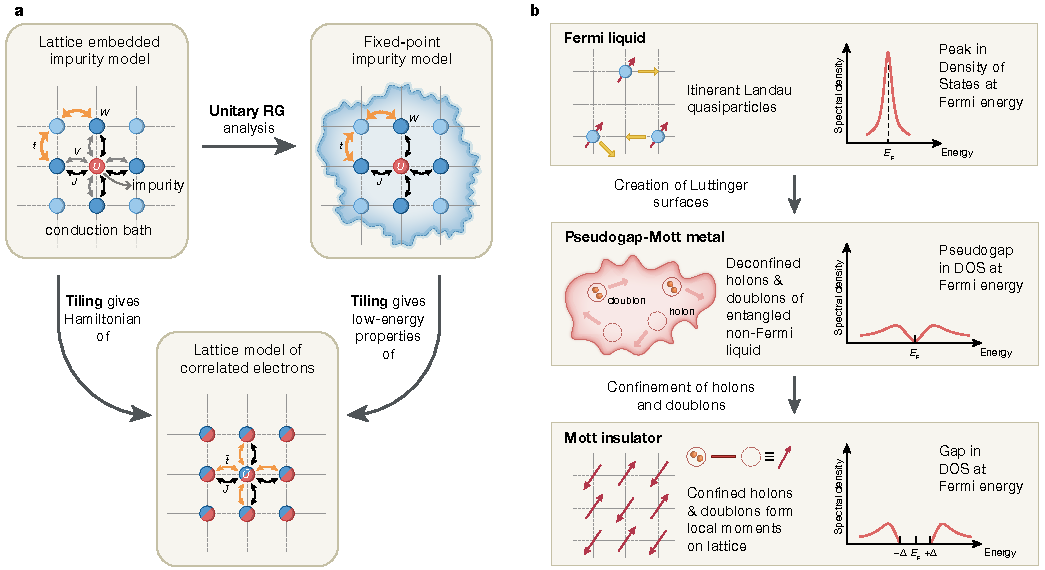
\includegraphics[scale=0.5]{schematic.png}
% }
% \only<2>{%
% \includegraphics[width=0.35\textwidth]{lm2sc.png}\\
% \hspace*{5pt}\includegraphics[width=0.35\textwidth]{fo2sc.png}
% }
% \end{tabular}
% \end{tabular}
\section{Summary of Results}
\begin{frame}[noframenumbering]{}
	\vspace*{-5pt}
	\begin{figure}[htpb]
		\centering
		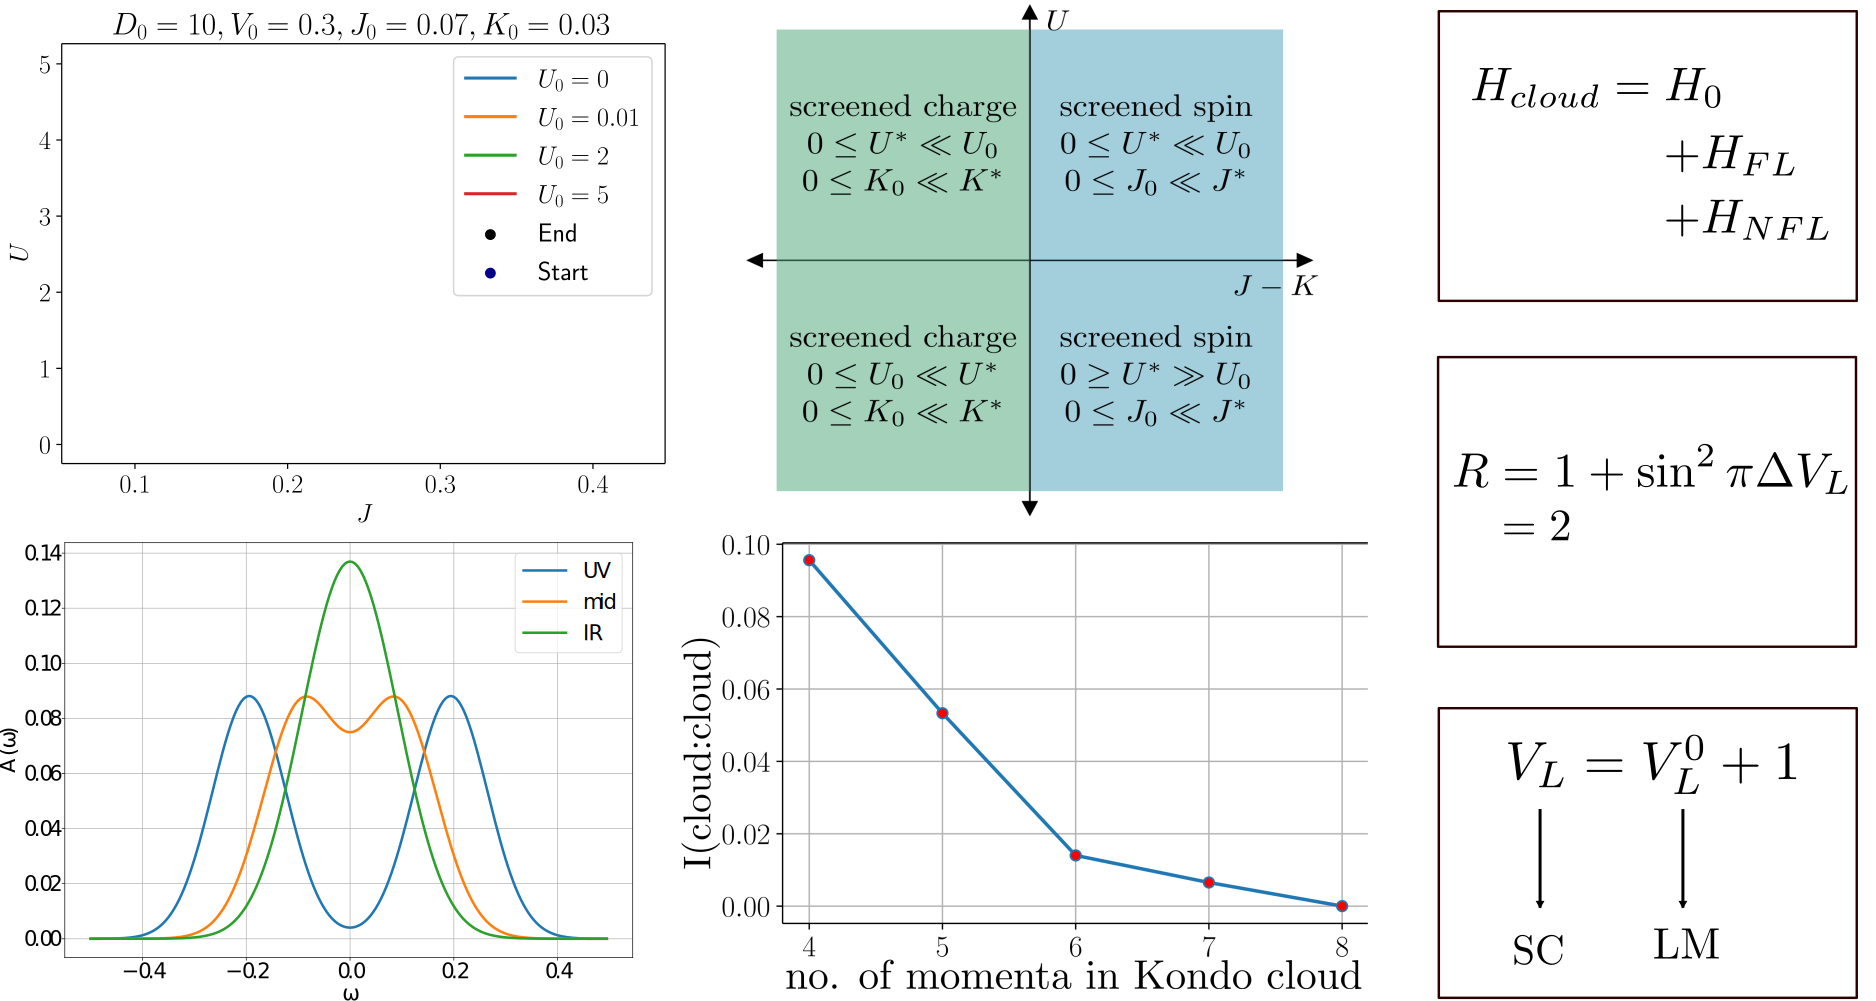
\includegraphics[width=\textwidth]{figures/summary.png}
	\end{figure}
\end{frame}

\section{Future Directions}
\begin{frame}[noframenumbering]{What's Next?}
\begin{itemize} 
\only<1-6>{\item Analytical expression for temperature-dependent Wilson ratio 
	\vspace{5pt}
}
\only<2-6>{\item Separating the contributions of various parts of the Kondo cloud to the spectral function
	\vspace{5pt}
}
\only<3-6>{\item Suggested by the generalized double-bracket form of URG, we can try to see if URG can be used as an optimizer.
	\vspace{5pt}
}
\only<4-6>{\item Since the zero-mode low-energy theory is an Anderson molecule (which can be exactly solved), it would be interesting to see if there is a transformation which converts the Anderson molecule to the Hubbard molecule.
	\vspace{5pt}
}
\only<5-6>{\item We can also check how using more feature-full baths (with non-trivial self-energy) can change the phase diagram.
	\vspace{5pt}
}
\only<6>{\item extensions to the Kondo and Anderson lattices, and hence to the problem of heavy Fermions
}
\end{itemize}
\end{frame}
\begin{frame}[noframenumbering]{}
	\cen{\LARGE Thanks for your attention!}

	\vspace*{\fill}
	\cen{\large{Special thanks to Dr. Siddhartha Lal, Siddhartha Patra, Dr. Anirban Mukherjee and Mounica Mahankali for guidance and feedback. The support of IISER Kolkata through a junior research fellowship is acknowledged.}}
\end{frame}
{\small \printbibliography}


\begin{frame}[noframenumbering]{URG: Relation to Poor Man's Scaling}
	\vspace*{-50pt}
	\cen{
		\Large\[H = H_0 + \underbrace{V_+ + V_-}_{\text{off-diagonal terms} \atop{\text{we want to remove}}}\]
}
\only<+>{
\begin{minipage}{0.45\textwidth}
\begin{figure}[htpb]
	\centering
	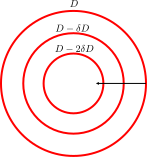
\includegraphics[width=0.7\textwidth]{figures/pms.png}
\end{figure}
\end{minipage}
\hspace*{20pt}
\begin{minipage}{0.45\textwidth}
Philosophy of Poor Man's scaling:
\begin{itemize}
	\item Successively eliminate high-energy energy shells
	\item Write high energy excitations as second-order correction to low-energy scatterings
	\item Typically perturbative
\end{itemize}
\end{minipage}
\footcite{Anderson}
}
\only<+>{
\hspace*{\fill}	\(E = \text{exact eigenvalue}\)\hspace*{\fill} \(\omega=\text{URG quantum fluctuation scale}\)\hspace*{\fill}

\vspace*{20pt}
\begin{minipage}{0.5\textwidth}
\[\Delta H_\text{PMS} = V_- \frac{1}{E - H_0}V_+ + V_+ \frac{1}{E - H_0}V_-\]
\cen{
	\large\(\Bigg\downarrow E \to \omega\)
}
\[\Delta H_\text{URG} = V_- \frac{1}{\omega - H_0}V_+ + V_+ \frac{1}{\omega - H_0}V_-\]
\end{minipage}
\begin{minipage}{0.49\textwidth}
\begin{figure}[htpb]
	\centering
	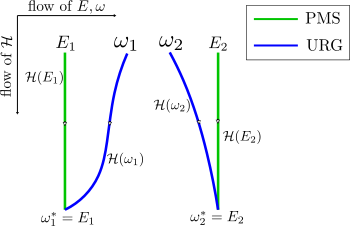
\includegraphics[width=0.9\textwidth]{figures/pms_vs_urg.png}
\end{figure}
\end{minipage}
}
\end{frame}
\begin{frame}[noframenumbering]{URG: Relation to Continuous Unitary Transformation RG}
\Large\[H = \overbrace{H_d}^\text{diagonal part} + \overbrace{H_X}^\text{off-diagonal part}\]
\cen{
	\Large$\Delta H_\text{CUT} = \Delta l\bigg[\big[H_d(l), H_X(l)\big], H(l)\bigg]$
}
\vspace*{20pt}
\only<+>{
	\begin{minipage}{0.39\textwidth}
		{\Large\(V_{kq}(l) = V_{kq}(0)e^{\left( \epsilon_k - \epsilon_q \right) l}\)}
\end{minipage}
\hspace*{0.09\textwidth}
\begin{minipage}{0.5\textwidth}
	\large{
	\begin{itemize}
		\item off-diagonal terms decay exponentially
			\vspace*{10pt}
		\item those that connect larger energy differences decay fastest
	\end{itemize}
}
\end{minipage}
\footcite{glazek-wilson,wegner_1994}
}
\only<+>{
	\vspace*{-10pt}
\cen{
	\large\(\Delta H_\text{URG} = \overbrace{\bigg[\big[H_d, \frac{1}{\omega_1 - \omega_0} \left( \hat \omega - H_d \right)^{-1} H_I\big], H\bigg]}^{\Delta H_0} - H^I\)\\[20pt]
	\large\(\Delta H_0 \xrightarrow{\left( \hat \omega - H_d \right)^{-1} \sim -H_d^{-1}} \Delta \lambda \times \bigg[\big[H_d, H_I\big], H\bigg]\)
}
}
\end{frame}
\end{document}
